% This LaTeX was auto-generated from MATLAB code.
% To make changes, update the MATLAB code and export to LaTeX again.

\documentclass{article}

\usepackage[utf8]{inputenc}
\usepackage[T1]{fontenc}
\usepackage{lmodern}
\usepackage{graphicx}
\usepackage{color}
\usepackage{listings}
\usepackage{hyperref}
\usepackage{amsmath}
\usepackage{amsfonts}
\usepackage{epstopdf}
\usepackage{matlab}

\sloppy
\epstopdfsetup{outdir=./}
\graphicspath{ {./ENTREGAVEL_parte3_images/} }

\begin{document}

\matlabtitle{Lista 1 - Parte 3}

\begin{par}
\begin{flushleft}
Autor: Francisco Castro
\end{flushleft}
\end{par}

\label{H_C24185FF}
\matlabheading{Introdução}

\begin{par}
\begin{flushleft}
    Este documento refere-se à implementação do algoritmo de Salichev incremental com quatro amostras, sendo a continuação (parte 3) das listas computacionais já entregues como atividade da disciplina EES-60, ministrada pelo Prof. Dr. Jacques Waldmann em 2019.
\end{flushleft}
\end{par}


\matlabheading{Método TRIAD}

\begin{par}
\begin{flushleft}
    Referente à Parte 1 da lista computacional.
\end{flushleft}
\end{par}

\begin{matlabcode}
metodoTRIAD;
\end{matlabcode}


\matlabheading{Estabilização vertical}

\begin{par}
\begin{flushleft}
    Implementado na Parte 2 com a finalidade de estabilizar o canal vertical dos sensores que, originalmente, produziam resultados extremamente divergentes. Assumindo-se a presença artificial de um altímetro de suporte, atribui-se o valor da altitude inicial como o valor de altitude medido por este a cada instante a fim de implementar a referida estabilização.
\end{flushleft}
\end{par}

\begin{par}
\begin{flushleft}
    Nesta, os ganhos $B$ e $C$ são determinados a fim de otimizar a oscilação e a divergência na altitude calculada de forma, por hora, empírica. Bem como a frequência da banda passante $T_h$, que foi arbitrariamente escolhida como 60, mas que, neste caso, não apresenta grande efeito nos resultados haja vista que atua sobre o sinal do sensor, visando minimizar ruídos.
\end{flushleft}
\end{par}

\begin{matlabcode}
h_m = h;
estabVert.B = 1;
estabVert.C = 1;
estabVert.T_h = 60;
\end{matlabcode}


\matlabheading{Modelamento da Terra e da gravidade}

\begin{par}
\begin{flushleft}
    Os parâmetros associados ao modelamento da Terra e da gravidade, $R_0$, $e$ e $g_0$ já foram definidos na chamada do Método TRIAD e são os que constam.
\end{flushleft}
\end{par}

\begin{matlabcode}
modTerra.R_0 = R_0; % [m]
modTerra.g_0 = g_0; % [m/s^2]
modTerra.e = e;     % achatamento
\end{matlabcode}

\begin{par}
\begin{flushleft}
    A saber
\end{flushleft}
\end{par}

\begin{matlabcode}
modTerra
\end{matlabcode}
\begin{matlaboutput}
modTerra = 
    R_0: 6378138
    g_0: 9.7803
      e: 0.0033529

\end{matlaboutput}


\matlabheading{Integração numérica}

\begin{par}
\begin{flushleft}
    Com isso, implementa-se o algoritmo de Salichev incremental com 4 amostras.
\end{flushleft}
\end{par}

\begin{matlabcode}
%% Preparação
tf = 19.5*60;               % tempo final
k0 = 36000/4;
i = 1;

freqAquisicao = 100;        % Hz
T = 1/freqAquisicao;        % passo de integração
result = zeros(tf/(4*T)-k0,12);

w_b = w_b.*T;               % Velocidade angular incremental
Asp_b = Asp_b.*T;           % Força específica incremental

%% Condições iniciais
q_NED_b = q0_base3;
V_NED = [0,0,0]';
lat = lambda;
lon = Lambda;
alt = h;
h_aux = h;

y = [...
    q_NED_b; ...
    V_NED; ...
    lat; ...
    lon; ...
    alt; ...
    h_aux ...
];

%% Integração
for k = k0:tf/(4*T)

    % Conjunto de 4 medidas
    omega_B_k = w_b(4*k-3 : 4*k-3+3, :)';
    Asp_B_k = Asp_b(4*k-3 : 4*k-3+3, :)';

    % Atualização de estado
    y = fs(k, y, omega_B_k, Asp_B_k, modTerra, estabVert, h_m, T);
    
    % Coleção de resultados
    result(i,1) = k*4*T;       % tempo [min]
    result(i,2:12) = y;        % vetor de estados
    i = i+1;
end
\end{matlabcode}


\matlabheading{Resultados}

\begin{par}
\begin{flushleft}
        Com isso, tem-se o seguinte resultado imediato da integração numérica
\end{flushleft}
\end{par}

\begin{matlabcode}
preProcessResults
\end{matlabcode}
\begin{center}
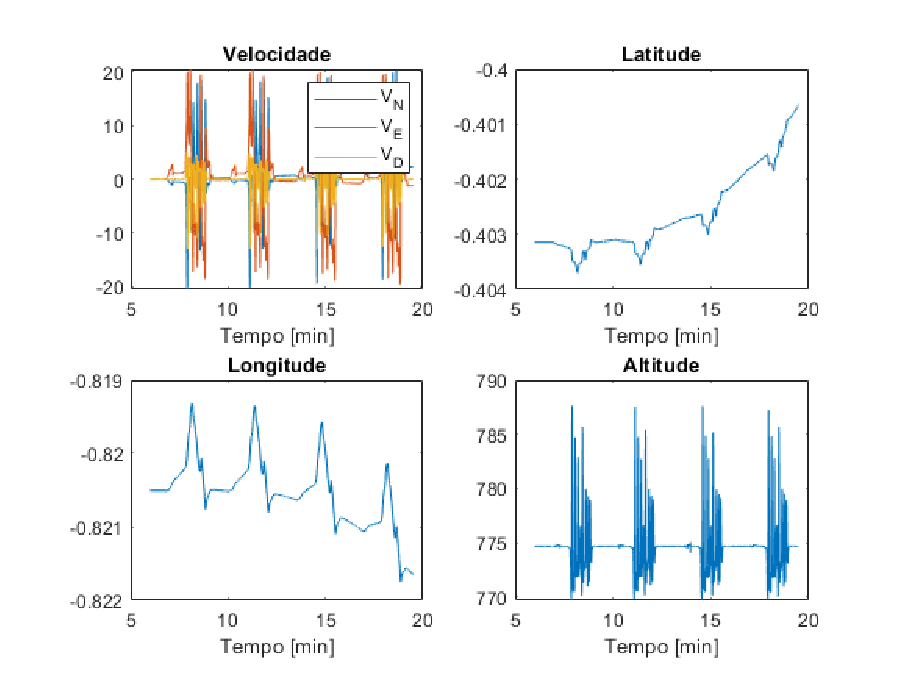
\includegraphics[width=\maxwidth{56.196688409433015em}]{figure_0}
\end{center}

\label{H_96BB6AB7}
\matlabheading{Análise da atitude computada pelo INS}

\begin{par}
\begin{flushleft}
\textbf{Vetor rotação}
\end{flushleft}
\end{par}

\begin{par}
\begin{flushleft}
    Calculou-se o vetor rotação ao final de cada volta com relação ao vetor original $q0$, em [arcseg], de forma que
\end{flushleft}
\end{par}

\begin{matlabcode}
format shortG;
rotacaoFinalDeVolta = [
vetorRotacao(resultados.quaternion(indexFim.volta1,:), q0_base3),...
vetorRotacao(resultados.quaternion(indexFim.volta2,:), q0_base3),...
vetorRotacao(resultados.quaternion(indexFim.volta3,:), q0_base3),...
vetorRotacao(resultados.quaternion(indexFim.volta4,:), q0_base3)...
]*180/pi*3600
\end{matlabcode}
\begin{matlaboutput}
rotacaoFinalDeVolta = 3x4    
      -8.3862      -26.509      -42.497      -5.1295
      -17.085       6.0036       55.061       38.791
      -34.109      -151.29      -223.67      -242.64

\end{matlaboutput}


\begin{par}
\begin{flushleft}
\textbf{Índice de desalinhamento ao final de cada volta (escala log)}
\end{flushleft}
\end{par}

\begin{par}
\begin{flushleft}
    Analogamente, temos que os índices de desalinhamento dos quatérnions ao final de cada volta com relação ao quatérnion inicial $q_0$ são dados, em [arcseg], por
\end{flushleft}
\end{par}

\begin{matlabcode}
indiceDesalFinalDeVolta = [
indiceDesalinhamento(resultados.quaternion(indexFim.volta1,:), q0_base3),...
indiceDesalinhamento(resultados.quaternion(indexFim.volta2,:), q0_base3),...
indiceDesalinhamento(resultados.quaternion(indexFim.volta3,:), q0_base3),...
indiceDesalinhamento(resultados.quaternion(indexFim.volta4,:), q0_base3)...
]*180/pi*3600
\end{matlabcode}
\begin{matlaboutput}
indiceDesalFinalDeVolta = 1x4    
        39.06       153.71       234.24       245.78

\end{matlaboutput}

\begin{par}
\begin{flushleft}
Que se fazem valores naturalmente crescentes e cada vez mais significativos ao estado atual e, consequentemente, à amplificação dos erros futuros devido ao erro nas condições iniciais a ser imposto no processo de integração numérica.
\end{flushleft}
\end{par}


\begin{par}
\begin{flushleft}
\textbf{Comparação: índice de desalinhamento [arcseg] com magnitude do desalinhamento [arcseg] computado com quaternions}
\end{flushleft}
\end{par}

\begin{matlabcode}
normasRotacao = [
    norm(rotacaoFinalDeVolta(:,1)),...
    norm(rotacaoFinalDeVolta(:,2)),...
    norm(rotacaoFinalDeVolta(:,3)),...
    norm(rotacaoFinalDeVolta(:,4))...
    ];
format shortE
comparacao1 = normasRotacao - indiceDesalFinalDeVolta
\end{matlabcode}
\begin{matlaboutput}
comparacao1 = 1x4    
   3.9565e-07  -1.2726e-08   6.3962e-08  -3.0984e-08

\end{matlaboutput}

\begin{par}
\begin{flushleft}
De onde vê-se que há uma alta concordância entre as duas métricas escolhidas para avaliar o desallinhamento do quaternion atual com relação ao quaternion inicial para cada fim de volta.
\end{flushleft}
\end{par}

\label{H_67BC192A}
\matlabheading{Análise da trajetória computada pelo INS}

\begin{par}
\begin{flushleft}
\textbf{Coordenadas geodésicas x cartesianas}
\end{flushleft}
\end{par}

\begin{matlabcode}
[xt,yt,zt] = geodToCart(...
    resultados.latitude,...
    resultados.longitude,...
    resultados.altitude,...
    modTerra);
\end{matlabcode}


\begin{par}
\begin{flushleft}
\textbf{Resultado da altura contra tempo}
\end{flushleft}
\end{par}

\begin{par}
\begin{flushleft}
\textbf{    }Se tomada em relação ao ponto inicial, temos que a altura em função do tempo, em metros, pode ser dada por:
\end{flushleft}
\end{par}

\begin{matlabcode}
figure;
plot(resultados.tempo/60, zt)
xlabel("Tempo [min]");
ylabel("Altura relativa [m]");
\end{matlabcode}
\begin{center}
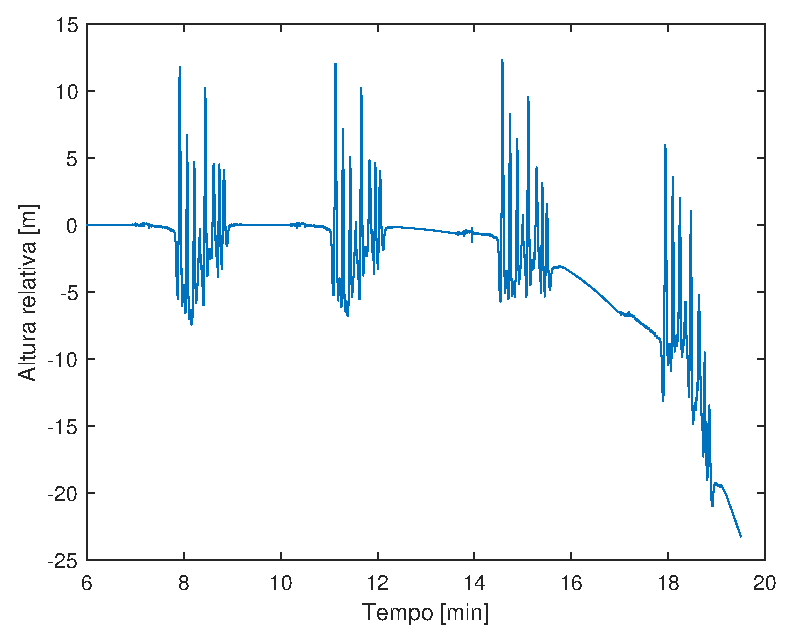
\includegraphics[width=\maxwidth{56.196688409433015em}]{figure_1}
\end{center}


\begin{par}
\begin{flushleft}
\textbf{Gráfico tri-dimensional da trajetória computada pelo INS}
\end{flushleft}
\end{par}

\begin{par}
\begin{flushleft}
     A trajetória estimada pelo INS em relação ao ponto inicial, em metros, nas direções Norte, Leste e altitude a partir do instante inicial 0[s], em relação ao ponto inicial, é tal que
\end{flushleft}
\end{par}

\begin{matlabcode}
figure;
plot3(xt,yt,zt)
\end{matlabcode}
\begin{center}
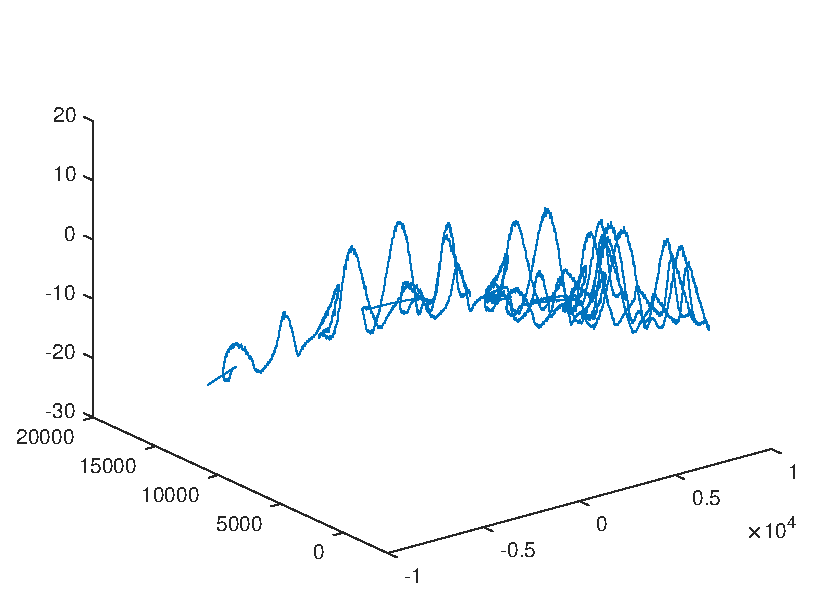
\includegraphics[width=\maxwidth{56.196688409433015em}]{figure_2}
\end{center}

\label{H_244DD4C2}
\matlabheading{Perguntas}

\begin{par}
\begin{flushleft}
    Nesta seção foram respondidas algumas das perguntas da Parte 2 que se faziam relevantes à alteração do algoritmo de integração.
\end{flushleft}
\end{par}

\begin{par}
\begin{flushleft}
\textbf{Quantas voltas há no primeiro experimento? Plote Norte contra Leste na primeira volta e superponha sobre a imagem (do Google Maps) de satélite da montanha russa Montezum do parque de diversões HopiHari em Vinhedo, SP, nas duas primeiras voltas e até o final do experimento. O que ocorre?}
\end{flushleft}
\end{par}

\begin{par}
\begin{flushleft}
    Há, no primeiro experimento, um total de 4 voltas. Que podem ser conferidas abaixo, onde se vê a superposição à foto real da montanha russa Montezum, retirada do Google Maps.
\end{flushleft}
\end{par}

\vspace{1em}

\begin{par}
\begin{flushleft}
\textbf{Figura 05. }Superposição do resultado da integração numérica com a imagem real para a primeira volta.
\end{flushleft}
\end{par}

\vspace{1em}

\vspace{1em}

\begin{par}
\begin{flushleft}
\textbf{Figura 06. }Superposição do resultado da integração numérica com a imagem real para as duas primeiras voltas.
\end{flushleft}
\end{par}

\vspace{1em}

\vspace{1em}

\begin{par}
\begin{flushleft}
\textbf{Figura 07. }Superposição do resultado da integração numérica com a imagem real para as quatro voltas.
\end{flushleft}
\end{par}

\vspace{1em}

\begin{par}
\begin{flushleft}
Observa-se, com isso, uma divergência crescente entre os resultados obtidos e o resultado esperado.
\end{flushleft}
\end{par}


\begin{par}
\begin{flushleft}
\textbf{Qual o erro de posição relativa ao ponto inicial no plano horizontal e em altura ao final da primeira volta no primeiro experimento?}
\end{flushleft}
\end{par}

\begin{matlabcode}
format shortg
erroHorizontal = sqrt(xt(indexFim.volta1)^2 + yt(indexFim.volta1)^2)
\end{matlabcode}
\begin{matlaboutput}
erroHorizontal = 
        81.99

\end{matlaboutput}
\begin{matlabcode}
erroAltura = zt(indexFim.volta1)
\end{matlabcode}
\begin{matlaboutput}
erroAltura = 
      0.01888

\end{matlaboutput}

\begin{par}
\begin{flushleft}
Note que a estabilização vertical vai ocasionar um erro de altura pequeno a depender do ganho a se colocar no controlador. Os resultados já estão em metros.
\end{flushleft}
\end{par}


\matlabheading{Apêndice}

\begin{par}
\begin{flushleft}
\textbf{Função de atualização de estado de Salichev}
\end{flushleft}
\end{par}

\begin{matlabcode}
function [y_new] = fs(t, y, omega_B_i, Asp_B_i, modTerra, estabVert, h_m, T)

    %% Preparação
    N = 1;
    E = 2;
    D = 3;

    R_0 = modTerra.R_0;
    e = modTerra.e;
    g_0 = modTerra.g_0;

    B = estabVert.B;
    C = estabVert.C;
    T_h = estabVert.T_h;

    Omega = 7.29e-5;

    %% Mapeamento de variáveis
    q_NEDold_bold = y(1:4);
    V_NED = y(5:7);
    lat = y(8);
    lon = y(9);
    alt = y(10);
    h_aux = y(11);
    
    %% Passo 0: quaternion de rotação do NEDold para NEDnew a cada 4 amostras de freqüência rápida dos sensores inerciais, computado com frequência lenta
    %% Modelo da Terra
    R_E = R_0*(1 + e*(sin(lat))^2);            % raio leste-oeste
    R_N = R_0*(1 - e*(2 - 3*(sin(lat))^2));    % raio norte-sul

    rho_NED = [...
        V_NED(E)/(R_E+alt), ...
        V_NED(N)/(R_N+alt), ...
        V_NED(E)/(R_E+alt)*tan(lat) ...
        ]';
    Omega_NED = [Omega*cos(lat),0,-Omega*sin(lat)]';

    omega_NEDi_NED = rho_NED + Omega_NED;  % taxa de transporte usa estimativas de velocidade terrestre e posição mais
     % recentes disponíveis 

    omega_versor = omega_NEDi_NED/norm(omega_NEDi_NED); % eixo de rotação instantânea unitário

    q_NEDold_NEDnew = [...
         cos(norm(omega_NEDi_NED*4*T)/2);...
         omega_versor(:)*sin(norm(omega_NEDi_NED*4*T)/2)
         ];

    %% Passo 1: incremento da velocidade de empuxo ?Uf ,b,k computada com frequência rápida. Índice k representa o instante inicial de um conjunto de 4 amostras; k+1 o instante inicial do próximo conjunto de 4 amostras, sem superposição com o anterior.
    alpha(:,1) = omega_B_i(:,1);
    alpha(:,2) = omega_B_i(:,2);
    alpha(:,3) = omega_B_i(:,3);
    alpha(:,4) = omega_B_i(:,4);

    delta_beta(:,1) = Asp_B_i(:,1);
    delta_beta(:,2) = Asp_B_i(:,2);
    delta_beta(:,3) = Asp_B_i(:,3);
    delta_beta(:,4) = Asp_B_i(:,4);

    W_k_0 = zeros(3,1);   % W_k(0) = (0,0,0)^T
    W_k_old = W_k_0;

    for m=1:4 % sculling correction
        W_k_new = delta_beta(:,m) - cross(alpha(:,m), W_k_old) + W_k_old;
        W_k_new = delta_beta(:,m) - cross(alpha(:,m), W_k_new) + W_k_old;
        W_k_old = W_k_new;
    end

    delta_U_f_b_k = W_k_new;

    %% Passo 2: Incremento angular computado com quatro amostras incrementais e quaternion de rotação bold qbnew do corpo na atitude anterior (bold) para o corpo na nova atitude (bnew). (new é a estampa de tempo k+1 e old é a estampa de tempo k) 
    % coning correction
    P1 = crossToMatrix(alpha(:,1));
    P2 = crossToMatrix(alpha(:,2));
    P3 = crossToMatrix(alpha(:,3));
    P4 = crossToMatrix(alpha(:,4));

    delta_phi = alpha(:,1)+alpha(:,2)+alpha(:,3)+alpha(:,4)+...
        2/3*(P1*alpha(:,2)+P3*alpha(:,4))+...
        1/2*(P1+P2)*(alpha(:,3)+alpha(:,4))+...
        1/30*(P1-P2)*(alpha(:,3)-alpha(:,4));

    delta_phi_versor = delta_phi/norm(delta_phi);

    q_bold_bnew = [...
         cos(norm(delta_phi)/2);...
         delta_phi_versor(:)*sin(norm(delta_phi)/2)
         ];

    % quaternion associado a ?Uf ,b,k
    delta_U_f_b_k_q = quat(delta_U_f_b_k);

    %% Passo 3: Computa em freqüência lenta o quaternion de rotação bnew qNEDnew mediante atualização de bold qNEDold devido à rotação de SNED para posterior transformação da força específica de Sb para SNED. (new é a estampa de tempo k+1 e old é a estampa de tempo k)
    q_NEDnew_bnew = quatInv(...
        quatProd(...
            quatProd(...
                quatInv(q_bold_bnew), ...
                quatInv(q_NEDold_bold)), ...
            q_NEDold_NEDnew)...
        );
    delta_U_f_NED_k_q = quatProd(...
        quatProd(...
            q_NEDnew_bnew, ...
            delta_U_f_b_k_q), ...
        quatInv(q_NEDnew_bnew)...
        );

    %% Passo 4: Atualiza em baixa freqüência (a cada período 4T) velocidade terrestre e posição. Usa posição ? k( ? ),1 k(h ? )1 e velocidade terrestre VNED,k?1 disponíveis para computar incremento de velocidade terrestre devido à gravidade.
    R_e = R_0*(1 - e*(sin(lat))^2);
    g = g_0*(1+.0053*(sin(lat))^2)*(1-2*alt/R_e);
    g_NED = [0,0,g]';

    delta_Vg_NED = (-cross((rho_NED + 2*Omega_NED), V_NED) + g_NED + [0,0,B*(alt-h_aux)]')*4*T;
    delta_V_NED = delta_Vg_NED + quatToVector(delta_U_f_NED_k_q);
    V_NED = V_NED + delta_V_NED;  %V_NED_new

    V_N = V_NED(N);
    V_E = V_NED(E);
    V_D = V_NED(D);

    % Atualizar lambda, Lambda e h para o instante k
    lat = lat + V_N/(R_N+alt);
    lon = lon + V_E/((R_E+alt)*cos(lat));
    alt = alt + -V_D - C*(alt-h_aux);
    h_aux = h_aux + (h_m-h_aux)/T_h;
    
    y_new = [...
        q_NEDnew_bnew; ...
        V_NED; ...
        lat; ...
        lon; ...
        alt; ...
        h_aux ...
    ];
end
\end{matlabcode}

\end{document}
